\section{Who Built the Stack}\label{sec:attribution}

A paper that measures someone else's software has to say early whose software it is. Before designing any experiment
we fetched every component at the commit the stack pins, applied every patch to its upstream, compared patches with
the pull requests they come from line by line, and searched every source tree for the code behind each feature
(\datafile{audit/ATTRIBUTION.md}, with the method in Section~\ref{sec:method} and the evidence under
\datafile{audit/evidence/}). Every model, kernel and placement algorithm in the stack comes from someone else, and each
layer depends on the one below it (Figure~\ref{fig:provenance}).

\begin{figure}[t]
\centering
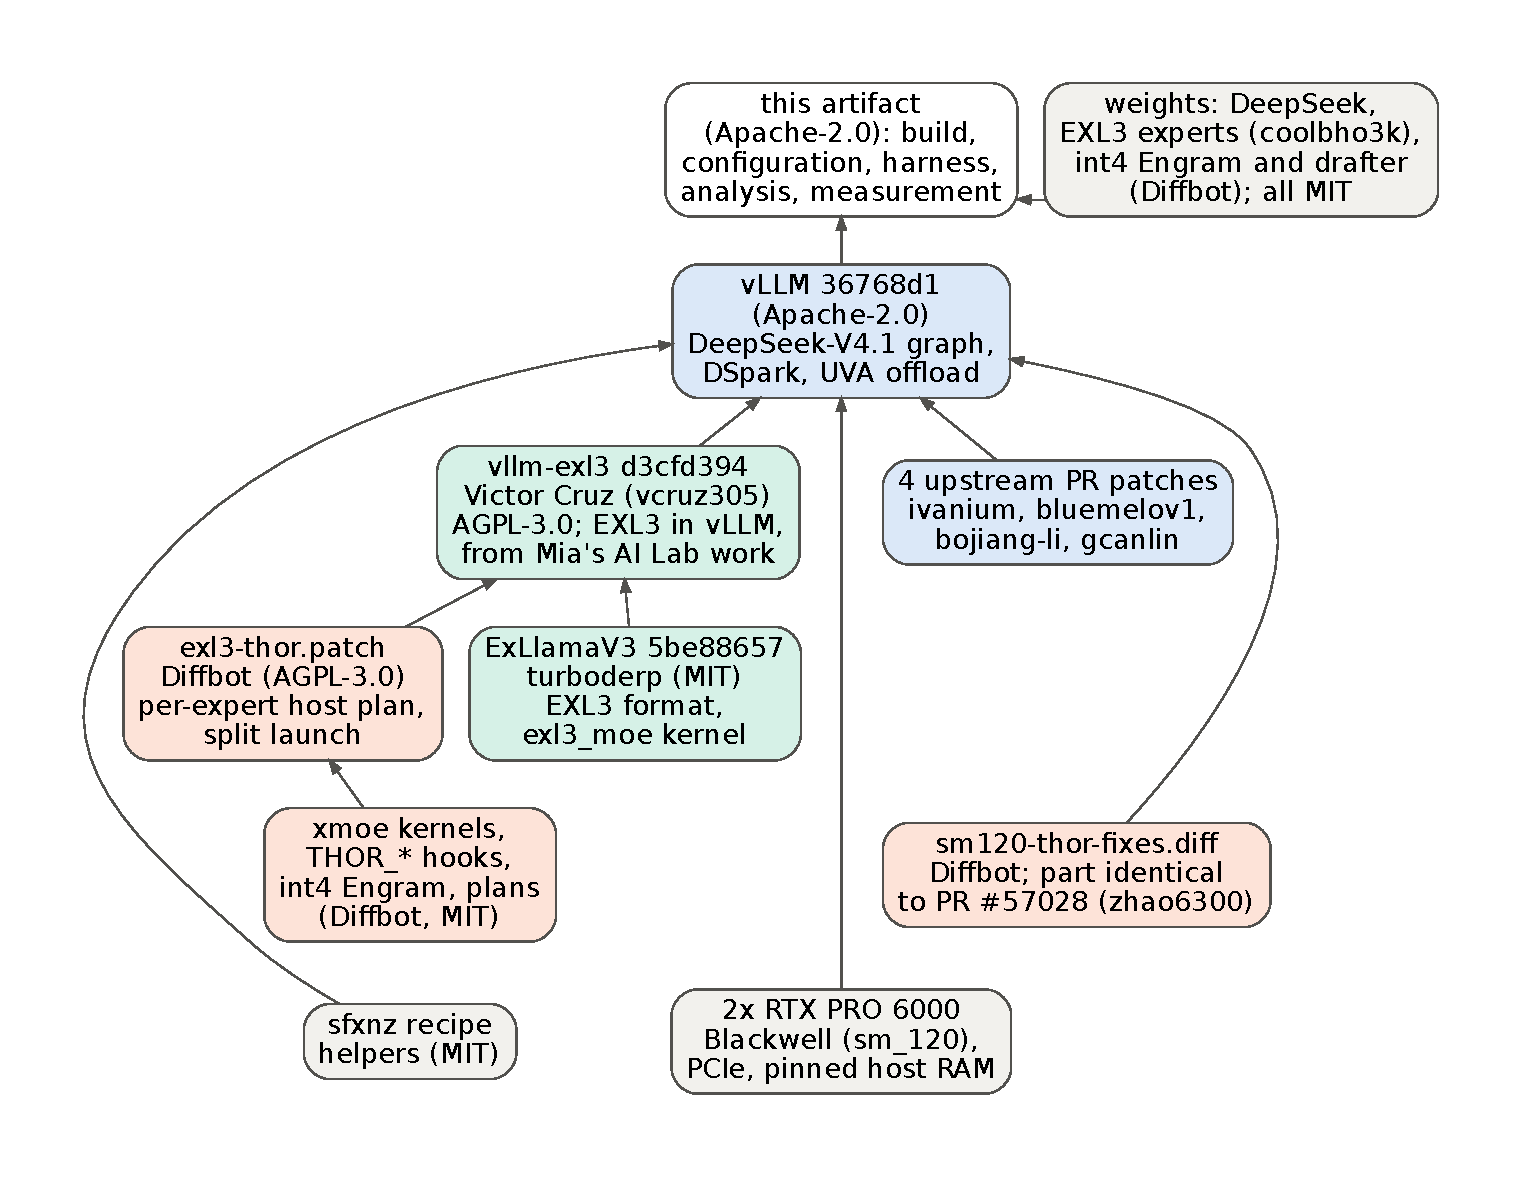
\includegraphics[width=\linewidth]{figures/generated/stack_provenance.pdf}
\caption{Layers of the measured stack and their authors (from \datafile{audit/ATTRIBUTION.md}, rendered from
\datafile{diagrams/stack_provenance.dot}). Orange: Diffbot's recipe. Blue: vLLM and upstream pull requests. Green:
EXL3 format and plugin.}
\label{fig:provenance}
\end{figure}

\paragraph{The people behind each layer.}
DeepSeek released the model's weights under the MIT license. turboderp wrote ExLlamaV3, its EXL3 weight format and the
\texttt{exl3\_moe} kernel that decodes compressed weights inside the matrix product, and coolbho3k quantized the
routed experts to \dv{cfg.exl3_bits} bits in that format. Victor Cruz (vcruz305) wrote vllm-exl3, the plugin that
brings EXL3 routed experts into vLLM, building on earlier work by Mia's AI Lab. That plugin is the foundation of the
whole arrangement. Diffbot's host-expert code is a patch to it, so none of the configurations we measure would run
without it. Diffbot wrote what makes the model fit: a plan file that lists, for every layer, which experts are cold
enough to live in host memory, chosen from routing counts over several traffic profiles, together with the kernels
and the split launch that compute those experts from host memory on a second CUDA stream while the hot experts run in
GPU memory. vLLM provides the serving engine, the DeepSeek-V4.1 graph, the DSpark speculative decoder and the
zero-copy reads of the Engram tables. Four upstream pull requests by ivanium, bluemelov1, bojiang-li and gcanlin, and
the runtime hooks of the sfxnz recipe, fill the remaining gaps. Table~\ref{tab:attribution} lists each feature with
its author and the class of contribution.

\paragraph{Three findings of the audit.}
First, the mechanism underneath the offload was not new inside the stack. Upstream vLLM at the pinned commit already
offers zero-copy weight offload with selection by parameter name, at the granularity of whole tensors, and Victor Cruz
documented an experimental placement of EXL3 expert payloads in pinned host memory two days after that commit and
before Diffbot's publication (\datafile{audit/evidence/vllm_upstream_offload.txt}). What Diffbot added is the
per-expert granularity, the profile-driven choice of which experts go out, and the kernels that make reading them
fast. Second, part of Diffbot's patch for the RTX PRO 6000's architecture (sm\_120) is identical to an open upstream
pull request by another author (zhao6300), which Diffbot's notices credit only in part. Third, our own share is small:
a build without docker, two serving settings (a larger maximum batch, and CUDA graph sizes capped low enough to avoid
a code path that graph capture cannot run), and everything that measures, from the load generator and the samplers to
the harness and the analysis (\datafile{audit/evidence/fat_any_item.txt}).

\begin{table}[t]
\centering\small
\begin{tabular}{p{4.3cm}p{3.4cm}p{3.4cm}l}
\toprule
feature & author & where & class \\
\midrule
DeepSeek-V4.1 graph, DSpark, Engram UVA offload, selective UVA weight offload & vLLM project & vLLM \texttt{36768d1} & implementation \\
EXL3 format and \texttt{exl3\_moe} kernel & turboderp & ExLlamaV3 \texttt{5be88657} & implementation \\
EXL3 support in vLLM & Victor Cruz (vcruz305), from Mia's AI Lab work & vllm-exl3 \texttt{d3cfd394} & implementation \\
EXL3 \dv{cfg.exl3_bits}-bit routed experts & coolbho3k & Hub checkpoint & artifact \\
per-expert host plan, split launch, side-stream SM budget & Diffbot & \texttt{exl3-thor.patch} & algorithmic + implementation \\
plan selection from routing counts & Diffbot & recipe \texttt{plans/} & heuristic \\
xmoe decode and decode-once prefill kernels & Diffbot (from ExLlamaV3) & recipe \texttt{kernels/} & implementation \\
int4 Engram format and lookup, host embedding, FP8 trims & Diffbot & recipe patches and hooks & implementation \\
sm\_120 fixes & Diffbot and zhao6300 (PR \#57028) & \texttt{sm120-thor-fixes.diff} & implementation \\
four upstream PR patches & ivanium, bluemelov1, bojiang-li, gcanlin & recipe \texttt{patches/vllm/} & implementation \\
runtime hooks & sfxnz, edited by Diffbot & \texttt{sitecustomize.py} & integration \\
build without docker, serve settings ($\le$64 sequences, graph sizes $\le$256) & inferencekey (us) & exploratory scripts & configuration \\
load generator, samplers, this harness and analysis & inferencekey (us) & this repository & measurement \\
\bottomrule
\end{tabular}
\caption{Authorship of the features measured in this paper, from the audit (\datafile{audit/ATTRIBUTION.md}, which gives
file:line evidence for every row). ``Class'' follows the audit's classification: algorithmic contribution,
implementation, integration, configuration, or measurement.}
\label{tab:attribution}
\end{table}

When this paper says ``the offload'', it means Diffbot's patch on top of upstream vLLM and Victor Cruz's plugin, run
with the recipe's own settings.
